\chapter{Background on x86 \& Windows}\label{chapter:background x86 windows}
We will first go over the necessary background information. In \autoref{section:background x86}, we give general information on the CPU architecture that is used by Windows, x86. As this provides information on general concepts (registers, memory management, and assembly), it can be skipped by people that are familiar with these subjects. After that, we will discuss function calls and how they work in assembly, in \autoref{section:function calls}. Finally, we will discuss Windows. As Windows is a large, complex platform and operating system, we will focus on concepts that are used in this thesis: the Windows API, the Windows Registry, Windows Services, and Scheduled Tasks.

In the next chapter we will discuss malware (\autoref{chapter:background malware}).

\section{The x86 Architecture}\label{section:background x86}
CPUs perform operations by executing instructions. The model that describes these instructions is called an \emph{instruction set architecture}. x86, an instruction set architecture developed by Intel, is the most widely used instruction set architecture \cite{x86-dominance}.

An instruction indicates what operation the CPU should perform on data, stored in \emph{registers} (\autoref{section:registers}) and in the computers' memory.

An important feature of an instruction set architecture is the size of the registers and memory addresses. For example, a 32-bit architecture means that the registers and memory addresses consist of 32 bits and can store $2^{32}$ different values. The 32-bit variant of the x86 architecture is called IA-32 (Intel Architecture, 32-bit). However, most modern systems use the 64-bit variant, x86-64. x86-64 has full backward compatibility with IA-32, meaning that applications compiled for IA-32 can run on x86-64 (as long as the operating system also supports running IA-32 binaries).


\subsection{Registers}\label{section:registers}
Registers are small storage units that a CPU uses to store data during computations. Registers are implemented on the CPU itself, making data access significantly faster than accessing data stored in memory. There are two types of registers: general purpose registers and special purpose registers.

\subsubsection{General-purpose Registers}
General-purpose registers are used to store data or a memory address (i.e. a pointer) to data. x86 (specifically IA-32) has eight general-purpose registers, each having a traditional purpose. However, most can also be used for other purposes.

\begin{itemize}
    \item \texttt{eax} (extended\footnote{32-bit registers are called ``extended'' to distinguish them from their 16-bit counterpart. For example, the 32-bit \texttt{eax} register and the 16-bit \texttt{ax} register.} accumulator register): Used in arithmetic operations.
    \item \texttt{ebx} (extended base register): Used as a pointer to data stored in memory.
    \item \texttt{ecx} (extended counter register): Stores the counter in looping operations.
    \item \texttt{edx} (extended data register): Used in I/O operations.
    \item \texttt{esi} (extended source index): Stores the address of the input data in certain operations on strings.
    \item \texttt{edi} (extended destination index): Stores the address of the output data in certain operations on strings.
    \item \texttt{ebp} (extended base pointer): Stores the address of the base of the current stack frame.
    \item \texttt{esp} (extended base stack pointer): Stores the address to the top of the stack.
\end{itemize}

In IA-32 these registers are larger versions of the registers used in the 16-bit and 8-bit variants of x86. For backward compatibility, x86 allows access to the 16-bit and 8-bit registers as the lower half of the 32-bit registers. Similarly, the 32-bit registers can be accessed in x86-64. \autoref{table:registers} shows how these register sizes relate to each other, using the \texttt{eax} register as an example.

\begin{table}[ht]
    \centering
    \begin{tabular}{|l|llllllll|}
        \hline
        \textbf{64-bit} & \multicolumn{8}{c|}{\texttt{rax}} \\ \hline
        \textbf{32-bit} & & & & \multicolumn{1}{l|}{} & \multicolumn{4}{c|}{\texttt{eax}} \\ \hline
        \textbf{16-bit} & & & & & & \multicolumn{1}{l|}{} & \multicolumn{2}{c|}{\texttt{ax}} \\ \hline
        \textbf{8-bit} & & & & & & \multicolumn{1}{l|}{} & \multicolumn{1}{l|}{\texttt{ah}} & \texttt{al} \\ \hline
    \end{tabular}
    \caption{The relation between the different accumulator registers in variants of x86.}
    \label{table:registers}
\end{table}

\subsubsection{Special Purpose Registers}
Besides the general-purpose registers, x86 also has registers that store specific information about the program state and the CPU state. Two important registers with a specific purpose are:
\begin{itemize}
    \item \texttt{eflags} (extended flags): Stores the data of previous instructions (e.g. the result of a comparison of two values) and the processor state as booleans.
    \item \texttt{eip} (extended instruction pointer): Stores the address of the next instruction.
\end{itemize}


\subsection{The Stack}\label{section:stack}
A \emph{stack} is a data structure to store elements. We can add elements to the stack and take elements from the stack, with the restriction that the element that was added last is always the first element that is taken from the stack. This makes a stack a LIFO (last in, first out) data structure. A stack has two operations:
\begin{itemize}
   \item \textbf{Push}: Add a new element on top of the stack.

   \item \textbf{Pop}: Remove the top (i.e. the most recently added) element from the stack.
\end{itemize}

x86 uses a stack in memory to store the state of function calls, called the \emph{call stack}. Each time a function is called, a \emph{stack frame} is pushed to the call stack. A stack frame stores the arguments, return address, and local variables of a function. When a function returns, the stack frame is popped from the stack.

The call stack grows downwards. When an application starts, the stack pointer is set to some address. When data is pushed on the stack, the stack pointer is \emph{decreased}. Likewise, when data is popped from the stack, the stack pointer is \emph{increased}.

\autoref{fig:stack} illustrates what the stack would look like if a function \texttt{f0} has called another function \texttt{f1}. As we can see, the call frame of the callee is at the top of the stack, on top of the stack frame of the caller.

\begin{figure}[ht]
   \centering
   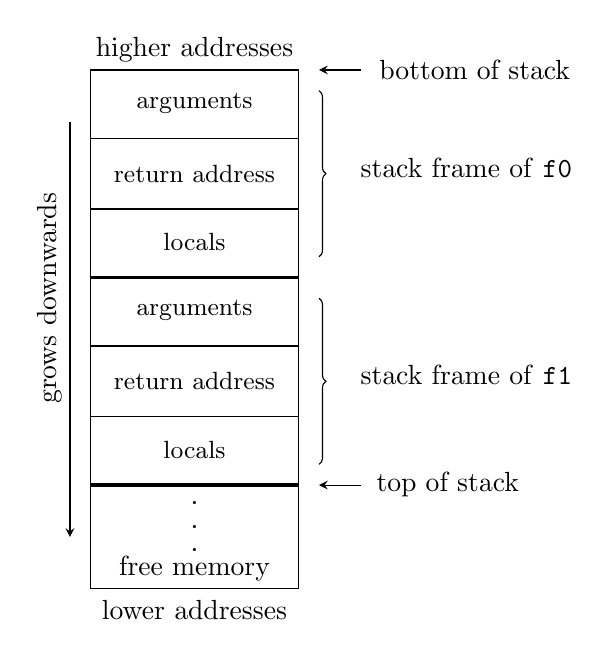
\begin{tikzpicture}[x=0.75pt,y=0.75pt,yscale=-1,xscale=1]

       % Arrow left of stack
       \draw (0,110) node[rotate=90] {grows downwards};
       \draw [-stealth] (10,25) -- (10,225) ;

       % Stack rectangle
       \draw (20,0) -- (120,0) -- (120,250) -- (20,250) -- cycle ;

       % Stack inside
       %% f0
       \draw (70,16) node {\small arguments};
       \draw (20,33) -- (120,33) ;
       \draw (70,50) node {\small return address};
       \draw (20,67) -- (120,67) ;
       \draw (70,83) node {\small locals};

       %% f1
       \draw [very thick] (20,100) -- (120,100) ;
       \draw (70,116) node {\small arguments};
       \draw (20,133) -- (120,133) ;
       \draw (70,150) node {\small return address};
       \draw (20,167) -- (120,167) ;
       \draw (70,183) node {\small locals};

       %% free memory
       \draw [very thick] (20,200) -- (120,200) ;
       \draw (70,220) node[rotate=90] {\large . . . };
       \draw (70,240) node {free memory};

       % Addresses
       \draw (70, -10) node {higher addresses};
       \draw (70, 260) node {lower addresses};

       %% Bottom of stack
       \draw [stealth-] (130,0) -- (150,0) ;
       \draw (205, 0) node {bottom of stack};

       %% Top of stack
       \draw [stealth-] (130,200) -- (150,200) ;
       \draw (192, 200) node {top of stack};

       %% Brace f0
       \draw [decorate, decoration={brace}] (130,10) -- (130,90) ;
       \draw (201,47) node {stack frame of \texttt{f0}};

       %% Brace f1
       \draw [decorate, decoration={brace}] (130,110) -- (130,190) ;
       \draw (201,147) node {stack frame of \texttt{f1}};
   \end{tikzpicture}
   \caption{The layout of the stack when \texttt{f0} has called \texttt{f1}.}
   \label{fig:stack}
\end{figure}

\medskip

Not all data of a program is stored on the stack. Larger and dynamically allocated data is stored in the \emph{heap}. Static and global variables are stored in a separate data segment.


\subsection{Assembly}\label{section:assembly}
Assembly is a low-level programming language in which, generally speaking, each statement corresponds to one instruction executed by the CPU. Assembly statements are compiled into byte sequences of machine code called \emph{opcodes}.

An assembly statement starts with the name of the instruction (the \emph{mnemonic}), followed by its operands (i.e. arguments). \autoref{listing:assembly example} shows an assembly statement where \texttt{mov} is the mnemonic and \texttt{eax} and \texttt{1} are the operands.

\begin{lstlisting}[caption={A single instruction moving the integer \texttt{1} into the register \texttt{eax}.}, label={listing:assembly example}, captionpos=b]
mov eax, 1
\end{lstlisting}

x86 assembly code is written in either Intel syntax (mostly used for Windows development) or AT\&T syntax (mostly used for Linux development). As we focus on Windows in this thesis, we will use the Intel syntax style.

In this section, we will discuss some basic instructions. There are, however, many more instructions used to efficiently perform operations on specific data types.

\subsubsection{Arithmetic Instructions}
x86 provides instructions for basic arithmetic.

\begin{itemize}
    \item \texttt{add op0, op1}: Add the value of \texttt{op1} to \texttt{op0}.
    \item \texttt{sub op0, op1}: Subtract the value of \texttt{op1} from \texttt{op0}.
    \item \texttt{imul op0, op1}: Multiply the value of \texttt{op0} with \texttt{op1} and store the result in \texttt{op0}.
    \item \texttt{idiv op0}: Divide the contents of \texttt{edx:eax} (a 64-bit value of which the 32 most significant bits are taken from \texttt{edx} and the 32 least significant bits are taken from \texttt{eax}) by \texttt{op0} and store the result in \texttt{eax}.
    \item \texttt{inc op0}: Increase the value of \texttt{op0} by 1.
    \item \texttt{dec op0}: Decrease the value of \texttt{op0} by 1.
\end{itemize}

\subsubsection{Logical Instructions}
x86 provides instructions for logical operations.

\begin{itemize}
    \item \texttt{and op0, op1}: Compute the bitwise and \texttt{op0} and \texttt{op1} and store the result in \texttt{op0}.
    \item \texttt{or op0, op1}: Compute the bitwise or of \texttt{op0} and \texttt{op1} and store the result in \texttt{op0}.
    \item \texttt{xor op0, op1}: Compute the bitwise exclusive or of \texttt{op0} and \texttt{op1} and store the result in \texttt{op0}.
    \item \texttt{not op0}: Compute the bitwise not of \texttt{op0} and store the result in \texttt{op0}.
\end{itemize}

\subsubsection{Data Movement Instructions}
x86 provides instructions for moving data between memory and registers.

\begin{itemize}
    \item \texttt{mov op0, op1}: Move the data stored in \texttt{op1} into \texttt{op0}.
    \item \texttt{lea op0, op1}: Move the address (i.e. pointer) stored in \texttt{op1} into \texttt{op0}.
\end{itemize}

\subsubsection{Stack Instructions}
x86 provides instructions for manipulating the call stack.

\begin{itemize}
    \item \texttt{push op0}: Push \texttt{op0} to the stack. This decreases the stack pointer. As pushing data to the stack is essentially writing the data to memory, \texttt{push eax} is equivalent to \autoref{listing:push with mov}.

\begin{lstlisting}[caption={The \texttt{push eax} instruction written in terms of \texttt{sub} and \texttt{mov}.}, captionpos=b, label={listing:push with mov}]
sub esp, 4
mov [esp], eax
\end{lstlisting}

    \item \texttt{pop op0}: Pop the top element from the stack and store it in \texttt{op0}. This increases the stack pointer. \texttt{pop eax} is equivalent to \autoref{listing:pop with mov}.

\begin{lstlisting}[caption={The \texttt{pop eax} instruction written in terms of \texttt{mov} and \texttt{add}.}, captionpos=b, label={listing:pop with mov}]
mov eax, [esp]
add esp, 4
\end{lstlisting}

\end{itemize}

\subsubsection{Control Flow Instructions}\label{section:control flow instructions}
x86 also provides instructions to control the flow of a program. This allows for subroutines (i.e. functions) to be defined and called. It also allows for conditional branching.

\begin{itemize}
    \item \texttt{call op0}: Call a subroutine defined at \texttt{op0}.

    A \texttt{call} performs two operations:
    \begin{enumerate}
        \item It pushes the address after the \texttt{call} instruction to the stack (This is the \emph{return address}).
        \item It changes the \texttt{eip} to the address that is being called (i.e. the next instruction will be at the address that is being called).
    \end{enumerate}

    If \texttt{op0} is an address, the call is \emph{direct}, because the function that is being called is known at compile time or load time. If \texttt{op0} is a register, the call is \emph{indirect} as the address to the function that is called is determined at runtime.

    \item \texttt{ret}: Signal the end of a subroutine and return to the caller. It pops the return address from the stack and jumps to it.
    \item \texttt{jmp op0}: Jump to the instruction at \texttt{op0}.
    \item \texttt{cmp op0, op1} and conditional jumps: It is possible to only jump if a condition is met. The \texttt{cmp} instruction compares the values of its two operands and stores the result in the special \texttt{eflags} register. A conditional jump instruction (e.g. \texttt{je op0}, \texttt{jne op0} and \texttt{jge op0}) reads this result and jumps if its specific condition is met. For example, \texttt{je op0} jumps to \texttt{op0} when the operands of \texttt{cmp} are equal.
\end{itemize}

Because of the control-flow instructions, assembly code is not sequential, but rather a graph structure that can loop and skip code. The code between two control flow instructions is run sequentially and called a \emph{basic block}. This creates a \emph{control flow graph} of basic blocks and paths between these blocks. The conditionals in the code decide which paths are taken. \autoref{fig:control flow graph} shows an example of the control flow graph of a function.

\begin{figure}[ht]
    \centering
    \includegraphics[width=0.9\textwidth]{resources/images/control_flow_graph.png}
    \caption{A screenshot from IDA Pro showing a control flow graph.}\label{fig:control flow graph}
\end{figure}


\section{Function Calls}\label{section:function calls}
Functions (sometimes called \emph{subroutines}) are an important part of modern programming languages. They allow splitting up code into reusable blocks. Functions can take inputs, called \emph{arguments}, and can return an output value. Executing the code in a function is done by \emph{calling} the function.

In C++ (and most other programming languages), function calls are expressed using the following format: \texttt{function\_name(arg 0, arg 1, ..., arg n)}. Function calls consist of the following \emph{function call elements}:
\begin{enumerate}
    \item The function name.
    \item The number of arguments.
    \item The value and type of each argument.
\end{enumerate}

For example, the function call \texttt{sum(1, 2)} to the function in \autoref{listing:sum function} tells us that:
\begin{enumerate}
    \item The function name is ``\texttt{sum}''.
    \item The function takes two arguments.
    \item The first argument is an \texttt{int}, \texttt{1}.
    \item The second argument is also an \texttt{int}, \texttt{2}.
\end{enumerate}

\begin{lstlisting}[label={listing:sum function}, caption={A C function that adds to integers together.}, captionpos=b]
int sum(int a, int b){
    return a + b;
}
\end{lstlisting}

\subsection{Calling Conventions}\label{section:calling conventions}
Functions are supported in assembly, through the \texttt{call} and \texttt{ret} instructions (discussed in \autoref{section:control flow instructions}). However, assembly does not explicitly support passing arguments to functions. Instead, arguments have to be stored in memory or registers before a function call such that the function will be able to access them. A \emph{calling convention} defines how arguments are passed to a function, on the assembly level. More specifically, a calling convention defines:
\begin{itemize}
    \item How arguments are passed to the callee. This can be on the stack, in registers, or both.
    \item The order in which arguments are passed to the callee.
    \item Whether the callee or caller cleans up the stack after the callee is finished.
    \item How return values are passed to the caller.
\end{itemize}

Calling conventions are specific to a function, which means that multiple calling conventions can be used throughout a single executable.

As we will see in \autoref{section:decompiling function calls}, calling conventions are important when analyzing function calls.

\medskip

There are many calling conventions in x86. We will discuss the three most prominent: cdecl, stdcall, and fastcall.

\subsubsection{Cdecl}\label{section:cdecl}
The cdecl\footnote{\tiny \url{https://docs.microsoft.com/en-us/cpp/cpp/cdecl?view=msvc-170}} convention is the default calling convention used by C. Arguments are pushed to the stack, right to left (i.e. the first argument is pushed to the stack last). The caller cleans up the stack. The return value is passed via \texttt{eax}.

The example C code and corresponding assembly\footnote{Compiled without any optimizations.} in \autoref{listing:sum cdecl} and \autoref{listing:main cdecl} shows cdecl in practice.

\begin{enumerate}
    \item \texttt{main} pushes the arguments to the stack (lines 7 and 9).
    \item \texttt{main} calls \texttt{sum} (line 10).
    \item \texttt{sum} runs and saves its result in \texttt{eax} (line 4).
    \item \texttt{main} cleans up the stack after the call (line 11), by lowering the top of the stack by 8 (the size of two integers).
\end{enumerate}

\begin{lstlisting}[label={listing:sum cdecl}, caption={The C code and assembly of a function that uses cdecl.}, captionpos=b]
int sum(int a, int b) { push    ebp
    return a + b;       mov     ebp, esp
}                       mov     eax, [ebp + 8]
                        add     eax, [ebp + 12]
                        pop     ebp
                        retn
\end{lstlisting}

\begin{lstlisting}[label={listing:main cdecl}, caption={The C code and assembly of a function calling the function from \autoref{listing:sum cdecl} using cdecl.}, captionpos=b]
int main() {            push    ebp
    int x = 1;          mov     ebp, esp
    int y = 2;          sub     esp, 8
    return sum(x, y);   mov     [ebp - 8], 1
}                       mov     [ebp - 4], 2
                        mov     eax, [ebp - 4]
                        push    eax
                        mov     ecx, [ebp - 8]
                        push    ecx
                        call    sum
                        add     esp, 8
                        mov     esp, ebp
                        pop     ebp
                        retn
\end{lstlisting}

\subsubsection{Stdcall}
The stdcall\footnote{\tiny \url{https://docs.microsoft.com/en-us/cpp/cpp/stdcall?view=msvc-170}} convention is used to call Win32 API functions. It is similar to cdecl, however, in stdcall, the callee cleans up the stack after it is done.

\subsubsection{Fastcall}
Fastcall\footnote{\tiny \url{https://docs.microsoft.com/en-us/cpp/cpp/fastcall?view=msvc-170}} is a calling convention designed by Microsoft. It is meant to offer a performance boost over cdecl and stdcall by passing some arguments via registers. The first two arguments that fit in a register are passed in \texttt{ecx} and \texttt{edx}, respectively. All other arguments are pushed to the stack right to left. In fastcall, the callee is responsible for cleaning up the stack after it is done.

In \autoref{listing:sum fastcall}, and \autoref{listing:main fastcall} we see C code and assembly similar to the code in \autoref{section:cdecl}. \texttt{sum} in \autoref{listing:sum fastcall} uses fastcall\footnote{This can be explicitly specified in C code by adding the fastcall keyword to the function declaration. For example, \texttt{int \_\_fastcall sum(int a, int b, int c)}.}.

\begin{enumerate}
    \item \texttt{main} stores the first two arguments to \texttt{edx} and \texttt{ecx} (lines 9 and 10).
    \item \texttt{main} pushes the third argument to the stack (line 8).
    \item \texttt{main} calls \texttt{sum} (line 11).
    \item \texttt{sum} runs and saves its result in \texttt{eax} (line 8).
    \item \texttt{sum} cleans up the stack (line 11) by lowering the top of the stack by 4 (the size of one integer). This implicitly happens in the \texttt{retn 4} instruction.
\end{enumerate}

\begin{lstlisting}[label={listing:sum fastcall}, caption={The C code and assembly of a function that uses fastcall.}, captionpos=b]
int sum(int a,int b,int c){ push    ebp
    return a + b + c;       mov     ebp, esp
}                           sub     esp, 8
                            mov     [ebp - 8], edx
                            mov     [ebp - 4], ecx
                            mov     eax, [ebp - 4]
                            add     eax, [ebp + 8]
                            add     eax, [ebp + 8]
                            mov     esp, ebp
                            pop     ebp
                            retn    4
\end{lstlisting}

\begin{lstlisting}[label={listing:main fastcall}, caption={The C code and assembly of a function calling the function from \autoref{listing:sum fastcall} using fastcall.}, captionpos=b]
int main() {                push    ebp
    int x = 1;              mov     ebp, esp
    int y = 2;              sub     esp, 12
    int z = 3;              mov     [ebp - 12], 1
    return sum(x, y, z);    mov     [ebp - 8], 2
}                           mov     [ebp - 4], 3
                            mov     eax, [ebp - 4]
                            push    eax
                            mov     edx, [ebp - 8]
                            mov     ecx, [ebp - 12]
                            call    sum
                            mov     esp, ebp
                            pop     ebp
                            retn
\end{lstlisting}

\subsection{Decompiling Function Calls}\label{section:decompiling function calls}
Compiling is the process of translating source code into executable machine code. \emph{Decompiling} is the reverse process: translating machine code back into source code. Decompilers are important in reverse engineering software (especially malware analysis), because, if done well, they allow a far better understanding of the functionality of an executable binary. As information about the source code is lost during compilation, it is often not possible to perfectly translate a binary into its source code. Decompilation often relies on heuristics to structure machine code into source code.

\medskip

In \autoref{chapter:plugin}, we will use a decompiler (from IDA Pro) to decompile function calls. As function calls are not standardized in assembly, decompiling function calls is a complex process, which is also heavily dependent on heuristics. When we find a \texttt{call} instruction that we want to decompile, there are two steps to reconstructing the function call:
\begin{enumerate}
    \item Determine the calling convention.

    As we discussed in \autoref{section:calling conventions}, there are various calling conventions that are commonly used (e.g. cdecl is the default calling convention in C++). However, compilers have total freedom in deciding how arguments are passed to a function in assembly and compilers for different programming languages often use custom calling conventions.

    The two important characteristics that differentiate calling conventions from one another are how arguments are passed and how the memory is cleaned up after the function call has finished. If we can discover how these two characteristics are implemented for a function call, we determine what calling convention is used.

    \item If we know the calling convention, we know how arguments are passed to the callee and in what order they are passed.

    We can use this information to backtrack from the \texttt{call} instruction and detect instructions that place data in the locations (i.e. registers or the stack) that are used to pass the arguments.

    For example, if we know that an argument is passed via the \texttt{ecx} register, we will look for instructions that store data in the \texttt{ecx} register.

    However, as arguments can be computed at runtime and compilers optimize memory usage, it is often impossible to reconstruct an argument.
\end{enumerate}

\subsubsection{An Example of Decompiling a Function Call}
Let's look at an example of decompiling a function call. \autoref{listing:call address sum} shows a simple example of a function call (to call the \texttt{sum} function in \autoref{listing:sum function}).

\begin{minipage}{0.9\textwidth}
\begin{lstlisting}[label={listing:call address sum}, caption={The C and assembly code of a function that calls \autoref{listing:sum function} (using cdecl).}, captionpos=b]
int main() {            push    ebp
    int x = 1;          mov     ebp, esp
    int y = 2;          sub     esp, 8
    return sum(x, y);   mov     [ebp - 8], 1
}                       mov     [ebp - 4], 2
                        mov     eax, [ebp - 4]
                        push    eax
                        mov     ecx, [ebp - 8]
                        push    ecx
                        call    <address>
                        add     esp, 8
                        mov     esp, ebp
                        pop     ebp
                        retn
\end{lstlisting}
\end{minipage}

\medskip

The first step is to determine the calling convention. We do this by answering how arguments are passed and whether the callee or the caller cleans up the stack.

How are arguments passed? In the instructions right before the \texttt{call instruction}, from lines 4 to 9, we see that two integers (\texttt{1} on line 4 and \texttt{2} on line 5) are pushed to the stack. This is a good indication that either cdecl or stdcall are used.

Does the callee or the caller clean up the stack? Right after the function call, on line 11, we see that the stack pointer is reduced by 8 bytes (the size of two integers). This tells us that the \texttt{main} function (i.e. the caller) cleans up the stack. A common calling convention that requires the caller to clean up the stack after a function call is cdecl.

By answering these two questions, we have determined that the calling convention cdecl is most likely used.

\medskip

The second step is to find the arguments that are passed to the function. As we noted earlier, we see that two integers are pushed to the stack (in the instructions on lines 4 to 9). Backtracking from the call signature, we first encounter 2 being pushed on the stack and after that we encounter 1 being pushed on the stack.

This tells us what the function call looks like \texttt{?(1, 2)}. The only part that we do not know is the function name. And because compilers often do not use function names from source code, we will not be able to reconstruct the function name.

If a callee is not part of the binary itself, but available in a library, the name might be available. We will discuss this in more detail in \autoref{section:dlls}.


\section{Windows}
In this thesis, we focus on malware that is made for Windows. In this section, we go over three parts of the Windows operating system that are important to malware.

\subsection{The Windows API}\label{section:background windows api}
To interact with the Windows operating system (e.g. write to a file), applications need to call functions provided by Windows. These functions (and related data structures) are collectively called the Windows API. The API is documented online\footnote{\tiny \url{https://docs.microsoft.com/en-us/windows/win32/api/_winprog/}}.

In \autoref{chapter:persistence techniques} and \autoref{chapter:call signatures}, we will see that malware calls specific API functions to achieve persistence.

\autoref{listing:windows API example} shows a simple example program that writes text to a file\footnote{The Windows API uses its own types to represent C types. For example, \texttt{DWORD} is the API type for a 32-bit unsigned integer.}. It calls three functions to interact with Windows: \texttt{CreateFile}\footnote{\tiny \url{https://docs.microsoft.com/en-us/windows/win32/api/fileapi/nf-fileapi-createfilew}}, \texttt{WriteFile}\footnote{\tiny \url{https://docs.microsoft.com/en-us/windows/win32/api/fileapi/nf-fileapi-writefile}} and \texttt{CloseHandle}\footnote{\tiny \url{https://docs.microsoft.com/en-us/windows/win32/api/handleapi/nf-handleapi-closehandle}}.

\begin{minipage}{0.9\textwidth}
\begin{lstlisting}[caption={An example of creating and writing to a file using the Windows API.}, captionpos=b, label={listing:windows API example}]
#include <iostream>
#include <windows.h>

int main() {
	HANDLE hFile;

	LPCWSTR filename = L"test.txt";
	LPCWSTR buffer = L"Hello World";
	DWORD szBuffer = wcslen(buffer) * sizeof(WCHAR);

	hFile = CreateFile(
		filename,
		GENERIC_WRITE,
		0,
		NULL,
		CREATE_ALWAYS,
		FILE_ATTRIBUTE_NORMAL,
		0);
	WriteFile(
		hFile,
		(LPVOID) buffer,
		szBuffer,
		0,
		NULL);
	CloseHandle(hFile);

	return 0;
}
\end{lstlisting}
\end{minipage}

\subsubsection{Dynamic-link Libraries}\label{section:dlls}
The functions in the Windows API are provided in dynamic-link libraries (DLLs), executables that do not run by themselves. They export functions that can be used by other applications. Dynamic-link libraries offer multiple advantages over statically linked libraries. Most notably, functions do not have to be compiled into every executable that uses them and need to be loaded into memory only once.

\subsubsection{Calling API Functions}\label{section:background calling api functions}
As we can see in \autoref{listing:windows API example}, Windows API functions are called like any other function. The process of matching a function call to the correct address is handled by Windows and transparent to developers.

Executables have an \emph{Import Address Table} (IAT), which is used to translate external function calls in the executable to the actual addresses of the functions in memory. When a function in a DLL is called, the \texttt{call} instruction jumps to an address in the IAT, which in turn jumps to the actual address of the function. At load-time (i.e. when an executable is loaded into memory before executing it), Windows adds the actual memory addresses of the functions to the IAT. This process is called \emph{load-time dynamic linking} \cite{load-time-dynamic-linking}.

It is also possible to load external functions at run-time (i.e. during the execution of an application), called \emph{run-time dynamic linking}. This requires developers to write their own code that finds the right address to a function at run-time. The Windows API provides two functions that help developers do this: \texttt{LoadLibrary} \footnote{\tiny \url{https://docs.microsoft.com/en-us/windows/win32/api/libloaderapi/nf-libloaderapi-loadlibrarya}} and \texttt{GetProcAddress}\footnote{\tiny \url{https://docs.microsoft.com/en-us/windows/win32/api/libloaderapi/nf-libloaderapi-getprocaddress}}. They work like this:

\begin{enumerate}
    \item \texttt{LoadLibrary} is called to get a handle on the DLL that contains the required function.
    \item \texttt{GetProcAddress} is called to search for the required function using the handle to the DLL.
\end{enumerate}

Malware authors prefer to load functions at run-time because the functions are not added to the IAT, which hides the external functions they make use of.

\subsubsection{A Comparison of Load-Time Dynamic Linking \& Run-time Dynamic Linking}\label{section:comparison load time run time dynamic linking}
\autoref{appendix:source code run time linking} contains the source code of two executables. The executables are semantically equivalent, but \autoref{listing:load-time dynamic linking code} uses direct function calls to Windows API and \autoref{listing:run-time dynamic linking code} uses run-time dynamic linking. Both executables perform the following steps:

\begin{enumerate}
    \item Open the Windows Registry key \path{HKLM\SOFTWARE\Microsoft\Windows NT\CurrentVersion}, by calling \texttt{RegOpenKeyEx}\footnote{\tiny \url{https://docs.microsoft.com/en-us/windows/win32/api/winreg/nf-winreg-regopenkeyexw}}.

    \item Get the data of the value \texttt{ProductName} in the Registry key, by calling \texttt{RegQueryValueEx}\footnote{\tiny \url{https://docs.microsoft.com/en-us/windows/win32/api/winreg/nf-winreg-regqueryvalueexw}}.

    \item Close the Registry key, by calling \texttt{RegCloseKey}\footnote{\tiny \url{https://docs.microsoft.com/en-us/windows/win32/api/winreg/nf-winreg-regclosekey}}.
\end{enumerate}

In \autoref{fig:call comparison}, we see the Assembly that is used to call \texttt{RegQueryValueEx} in both executables. We can see that the disassembler detected which function is being called in \autoref{fig:load-time linked API call}, but not in \autoref{fig:run-time linked API call}. The \texttt{call} instruction in \autoref{fig:run-time linked API call} does not jump to a static address, but to an address that is loaded into the \texttt{eax} register.

\begin{figure}[ht]
    \centering
    \begin{subfigure}[ht]{\textwidth}
        \centering
        \includegraphics[width=0.7\textwidth]{resources/images/load_time_api_call_disassembler.png}
        \caption{A (load-time dynamically linked) call to \texttt{RegOpenKeyExW} (disassembled by IDA Pro).}
        \label{fig:load-time linked API call}
    \end{subfigure}
    \hfill
    \begin{subfigure}[ht]{\textwidth}
        \centering
        \includegraphics[width=0.7\textwidth]{resources/images/run_time_api_call_disassembler.png}
        \caption{A run-time dynamically linked call to \texttt{RegOpenKeyExW} (disassembled by IDA Pro).}
        \label{fig:run-time linked API call}
    \end{subfigure}
    \caption{A comparison of a load-time dynamically linked call and a run-time dynamically linked call to \texttt{RegOpenKeyExW}.}
    \label{fig:call comparison}
\end{figure}

In \autoref{fig:imports comparison}, we see part of the import table (decoded by IDA Pro) of the two executables. In \autoref{fig:load-time imports}, we see the three API functions, as expected. However, in \autoref{fig:run-time imports} we do not see the API functions, because the executable loads the functions itself.

\begin{figure}[ht]
    \centering
    \begin{subfigure}[ht]{\textwidth}
        \centering
        \includegraphics[width=0.7\textwidth]{resources/images/load_time_api_call_imports.png}
        \caption{The imports of \autoref{listing:load-time dynamic linking code} using load-time dynamically linked calls.}
        \label{fig:load-time imports}
    \end{subfigure}
    \hfill
    \begin{subfigure}[ht]{\textwidth}
        \centering
        \includegraphics[width=0.7\textwidth]{resources/images/run_time_api_call_imports.png}
        \caption{The imports of \autoref{listing:run-time dynamic linking code} using run-time dynamically linked calls.}
        \label{fig:run-time imports}
    \end{subfigure}
    \caption{A comparison of the import address table of two executables.}
    \label{fig:imports comparison}
\end{figure}

\subsection{The Windows Registry}\label{section:background windows registry}
The Windows Registry\footnote{\tiny \url{https://docs.microsoft.com/en-us/windows/win32/sysinfo/registry}} is a database of configuration settings for both the OS and applications. It is used to store almost all settings of the Windows operating system (e.g. the current Windows Version and the configuration of each service).

Malware uses the Registry as a source of information (e.g. to find the current version of the OS) and to achieve persistence\footnote{Fileless malware, a type of malware that does not depend on executable files, often uses the Registry to store its executable code \cite{fileless-malware}.} (as we see in \autoref{section:registry-based persistence}).

\subsubsection{The Structure of the Windows Registry}
The Registry has a tree-hierarchy that consists of \emph{keys} and \emph{values}. A key stores other keys (referred to as \emph{subkeys}) and values. Values are a combination of a name, data, and the type of the data, similar to files. A path of subkeys is referenced using a backslash as a delimiter, similar to Windows directory paths.

\medskip

Let's look at an example Registry key: \path{HKEY_LOCAL_MACHINE\SOFTWARE\Microsoft\Windows NT\CurrentVersion}. This path contains five keys: \path{HKEY_LOCAL_MACHINE}, \path{SOFTWARE}, \path{Microsoft}, \path{Windows NT} and \path{CurrentVersion}. \path{SOFTWARE} is a subkey of \path{HKEY_LOCAL_MACHINE}, \path{Microsoft} is a subkey of \path{SOFTWARE}, etc.

\medskip

Registry paths always start with a root key. There are five root keys:
\begin{itemize}
    \item \texttt{HKEY\_LOCAL\_MACHINE} (\texttt{HKLM}): Stores settings that apply to the whole operating system and all users.
    \item \texttt{HKEY\_USERS} (\texttt{HKU}): Stores user-specific settings. The direct subkeys of \texttt{HKU} are the identifiers of each user.
    \item \texttt{HKEY\_CURRENT\_USER} (\texttt{HKCU}): A virtual key that points to the subkey of the current user in \texttt{HKU}.
    \item \texttt{HKEY\_CURRENT\_CONFIG} (\texttt{HKCC}): Stores information on the current hardware configuration.
    \item \texttt{HKEY\_CLASSES\_ROOT} (\texttt{HKCR}): Stores information on file extension associations.
\end{itemize}

The most important root keys for malware are \texttt{HKLM} and \texttt{HKCU}, as they contain the most useful information and control the most useful settings (e.g. which executables are automatically started at boot time).

\subsubsection{CRUD Operations on the Windows Registry}
There are multiple ways to interact with the Windows Registry (i.e. perform CRUD\footnote{CRUD stands for the four basic operations on databases and storage: Create, Read, Update and Delete.} operations on the Windows Registry):
\begin{itemize}
    \item The Windows API: The Windows API exposes multiple functions that can be used to read or manipulate the Registry. For example, \texttt{RegOpenKeyEx} and \texttt{RegQueryValueEx} used in \autoref{section:comparison load time run time dynamic linking}.

    \item Registry Editor: Windows provides a GUI application that users can use to view and change the Registry.

    \item \texttt{reg.exe} commands\footnote{\tiny \url{https://docs.microsoft.com/en-us/windows-server/administration/windows-commands/reg}}: Windows also provides a command-line application that can be used to view and change the Registry from the command line.

    \item \texttt{.reg} files: Windows support special script-like files that contain values for Registry keys. When these are executed, Windows automatically changes the Registry. \autoref{listing:reg file example} shows the contents of an example \texttt{.reg} file.

    \begin{lstlisting}[caption={An example \texttt{.reg} file.}, captionpos=b, label={listing:reg file example}]
    Windows Registry Editor Version 5.00

    [HKLM\SOFTWARE\Microsoft\Windows\CurrentVersion\Run]
    "startup value"="C:\Windows\System32\cmd.exe"
    \end{lstlisting}
\end{itemize}

Malware most often uses the Windows API to edit the Registry directly \cite{practical-malware-analysis}.

As some registry values control global settings or settings that impact security, many keys require administrative privileges to change (e.g. all keys under \texttt{HKLM}).

\subsection{Scheduled Tasks \& Services}\label{section:scheduled tasks services in windows}
Windows supports running processes in the background without user interaction. This is useful for processes that should always be active, but do not require user interaction (e.g. antivirus software or hardware drivers). As we will see in \autoref{section:service-based persistence} and \autoref{section:scheduled task-based persistence}, malware also uses background tasks for persistence.

A Windows service\footnote{\tiny \url{https://docs.microsoft.com/en-us/windows/win32/services/services}} is a process that is started automatically when a Windows system is started (or other another Windows event happens) and runs in the background. Services can run even before a user has logged in, because they can run under the privileges of special system users.

Scheduled Tasks\footnote{\tiny \url{https://docs.microsoft.com/en-us/windows/win32/taskschd/task-scheduler-start-page}} are similar to services. A scheduled task starts an application at a specific event (e.g. when a user logs in), at a pre-defined time, or on a repeating schedule, without any user interaction.

Services and Scheduled Tasks can run as any user account. However, as some services need to run even when no user is logged in, they can also run as one of three special accounts\footnote{\tiny \url{https://docs.microsoft.com/en-us/windows/win32/services/service-user-accounts}}:
\begin{itemize}
    \item \texttt{LocalService}\footnote{\tiny \url{https://docs.microsoft.com/en-us/windows/win32/services/localservice-account}}: An account with minimal privileges.

    \item \texttt{NetworkService}\footnote{\tiny \url{https://docs.microsoft.com/en-us/windows/win32/services/networkservice-account}}: An account with minimal privileges with permission to authenticate to remote servers.

    \item \texttt{LocalSystem}\footnote{\tiny \url{https://docs.microsoft.com/en-us/windows/win32/services/localsystem-account}}: An account with full privileges on the local machine. This account is especially interesting to malware, as it grants full control of the machine.
\end{itemize}

Creating a service or scheduled task requires Administrator privileges, as they can be started using the \texttt{LocalSystem} user, which grants full control of the host.

\subsubsection{Creating Services}
There are multiple ways to create a service:
\begin{itemize}
    \item Windows provides a GUI (called ``Services'') that Administrator users can use to create, list, and modify services.

    \item The Windows API provides a function to create a Windows service: \texttt{CreateService}\footnote{\tiny \url{https://docs.microsoft.com/en-us/windows/win32/api/winsvc/nf-winsvc-createservicea}}.

    \item Windows provides a command-line application (\texttt{sc.exe}\footnote{\tiny \url{https://docs.microsoft.com/en-us/windows/win32/services/configuring-a-service-using-sc}}) that allows users with Administrator privileges to create services from the command line.

    \item Like most configuration settings on Windows, the configuration of services is stored in the Registry. The configuration of services is stored in the key \path{HKLM\SYSTEM\CurrentControlSet\services}.
\end{itemize}

\subsubsection{Creating Scheduled Tasks}
There are multiple ways to create scheduled tasks in Windows:
\begin{itemize}
    \item The Windows Task Scheduler is a GUI interface that Administrator users can use to create, list, and modify scheduled tasks.

    \item It is possible to create a scheduled task with the Windows API\footnote{\tiny \url{https://docs.microsoft.com/en-us/windows/win32/taskschd/daily-trigger-example--c---}}. To do this, one first needs to connect to the service used by the Scheduled Tasks. This is done using the \texttt{CoCreateInstance}\footnote{\tiny \url{https://docs.microsoft.com/en-us/windows/win32/api/combaseapi/nf-combaseapi-cocreateinstance}} function. This function is called with \texttt{CLSID\_TaskScheduler} as its first argument and \texttt{IID\_ITaskService} as its fourth.

    \item \texttt{schtasks.exe}\footnote{\tiny \url{https://docs.microsoft.com/en-us/windows/win32/taskschd/schtasks}} is a command-line application that allows users with Administrator privileges to create Scheduled Tasks from the command line.

    \item The predecessor of \texttt{schtasks.exe} is \texttt{at.exe}\footnote{\tiny \url{https://docs.microsoft.com/en-us/windows-server/administration/windows-commands/at}}. It works similarly to \texttt{schtasks.exe}, in that it can be used to create Scheduled Tasks from the command line. Although it is deprecated, it is still available.
\end{itemize}


